\chapter{Анализ и контроль показателей качества электрической энергии в электроэнергетических системах}\label{ch:ch1}

В первом разделе рассматривается понятие, характеризующее КЭ в электрических сетях систем электроснабжения переменного тока с частотами 50 и 60~Гц и порядок оценки результатов. Стандарты в области контроля определяющие состав показателей качества электрической энергии, методику измерений и характеристики средств измерений. В результате анализа производится сравнение государственных стандартов Российской Федерации и международных стандартов (МЭК, IEC – International Electrotechnical Commission), которые описывают требования и нормы КЭ \cite{IEC}.
%\hyperlink{https://www.iec.ch/}{[199]}. 
% [199 - International Electrotechnical Commission [Электронный ресурс] – Режим доступа:https://www.iec.ch/]

В первом разделе произведен сравнительный анализ существующих средств контроля учета показателей КЭ. В заключении описывается основные задачи и виды контроля КЭ.

\section{Понятие качества электрической энергии}\label{sec:ch1/sec1_1}
Повышение КЭ является основным фактором улучшения энергетической эффективности промышленных предприятий \cite{закон2009энергосбережении}. 
% [10 - Закон Ф. Об энергосбережении и о повышении энергетической эффективности и о внесении изменений в отдельные законодательные акты Российской Федерации //№ 261-ФЗ от 23.11. – 2009.]
%http://www.consultant.ru/document/cons_doc_LAW_93978/

Понятие качества электрической энергии (КЭ) описано ГОСТ 32144–2013~\cite{ГОСТ32144-2013} п.3.1.38, обозначает степень соответствия характеристик электрической энергии в данной точке электрической системы совокупности нормированных показателей КЭ.
% [125 - ГОСТ 32144-2013 Электрическая энергия. Совместимость технических средств электромагнитная. Нормы качества электрической энергии в системах электроснабжения общего назначения [Электронный ресурс] – Режим доступа: http://docs.cntd.ru/document/1200104301/]

Задача исследования – улучшить показатели качества электрической энергии (ПКЭ) в электрических сетях систем электроснабжения, совершенствуя средства измерительных устройств для определения гармоник. При разработке технического устройства должны учитываться ПКЭ  согласно действующим нормативам. 

Введен целый ряд нормативных документов (МЭК, ГОСТ). Изменение стандартов в области измерений электрической энергии показано на рисунке.
\cite{ГОСТ30804.4.30-2013, ГОСТ30804.4.7-2013, ГОСТ32144-2013, ГОСТР8.655-2009, ГОСТР51317.4.15-2012,ГОСТ33073-2014,ГОСТ8.622-2013} 
 
\begin{figure}[ht]
	\centerfloat{
		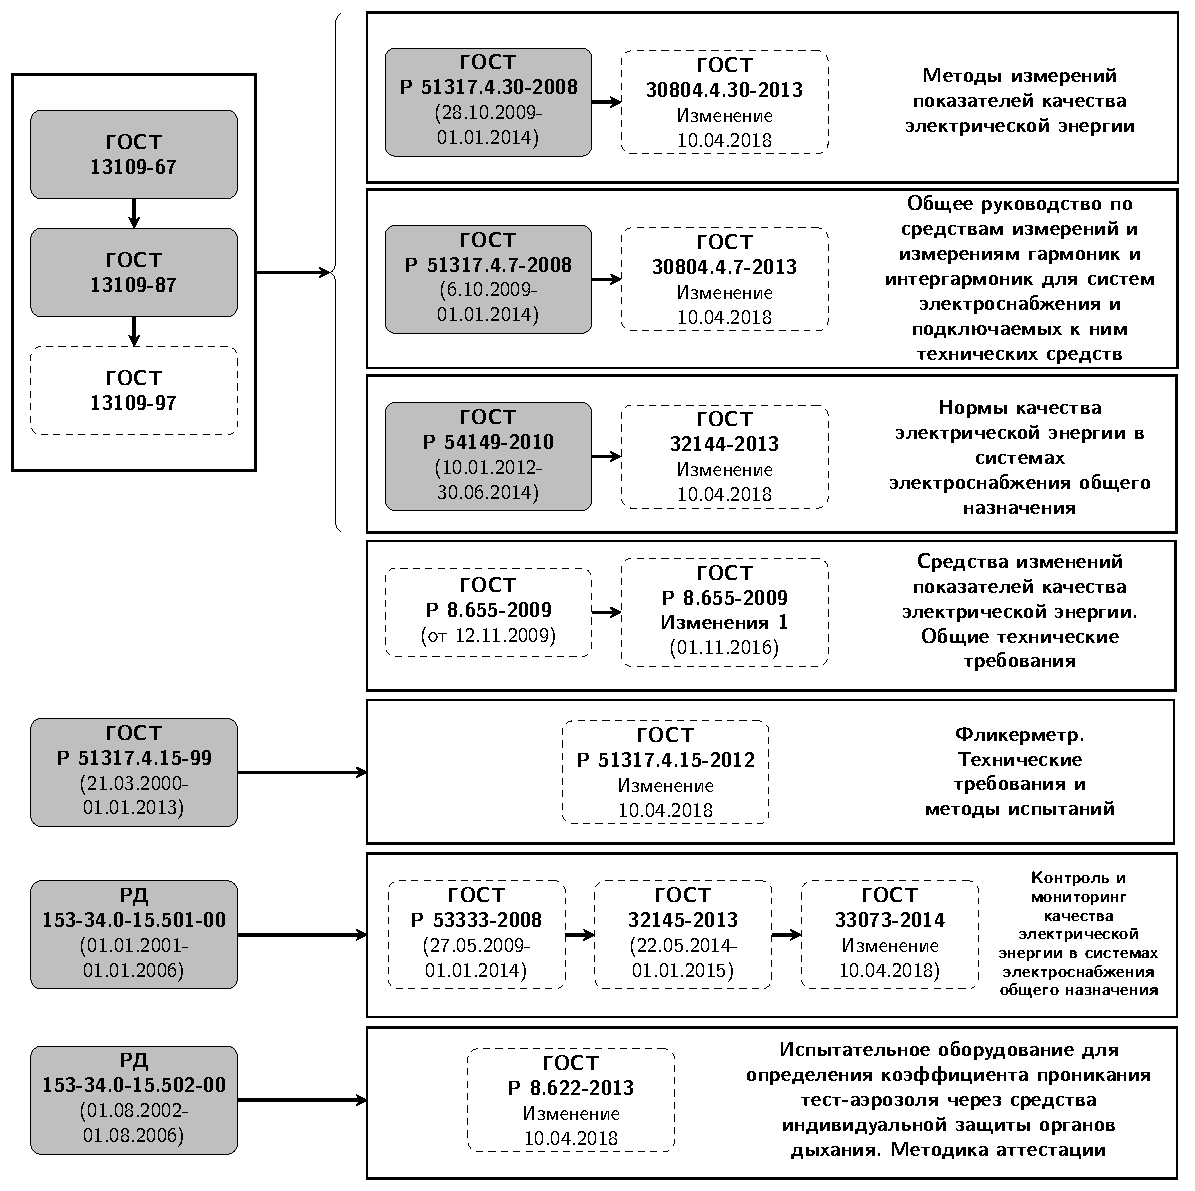
\includegraphics[scale=0.7]{picture1}
	}
	\caption{Развитие государственных стандартов в области контроля КЭ.}\label{fig:picture1}
\end{figure}
%Действующие стандарты на рисунке

% [179 - ГОСТ 30804.4.30-2013 (IEC 61000-4-30:2008) Электрическая энергия. Совместимость технических средств электромагнитная. Методы измерений показателей качества электрической энергии (с Поправкой) [Электронный ресурс] / Режим доступа: http://docs.cntd.ru/document/1200104665]

% [4 - ГОСТ 30804.4.7-2013 (IEC 61000-4-7:2009) Совместимость технических средств электромагнитная. Общее руководство по средствам измерений и измерениям гармоник и интергармоник для систем электроснабжения и подключаемых к ним технических средств (с Поправкой) [Электронный ресурс] / Режим доступа: http://docs.cntd.ru/document/1200103652]

% [125 - ГОСТ 32144-2013 Электрическая энергия. Совместимость технических средств электромагнитная. Нормы качества электрической энергии в системах электроснабжения общего назначения [Электронный ресурс] – Режим доступа: http://docs.cntd.ru/document/1200104301/]

% [136 - ГОСТ Р 8.655-2009 Государственная система обеспечения единства измерений (ГСИ). Средства измерений показателей качества электрической энергии. Общие технические требования (с Изменением N 1) [Электронный ресурс] / Режим доступа: http://docs.cntd.ru/document/1200075494/]

% [194 - ГОСТ Р 51317.4.15-2012 (МЭК 61000-4-15:2010) Совместимость технических средств электромагнитная. Фликерметр. Функциональные и конструктивные требования [Электронный ресурс] / Режим доступа: http://docs.cntd.ru/document/1200096463]

% [195 - ГОСТ 33073-2014 Электрическая энергия. Совместимость технических средств электромагнитная. Контроль и мониторинг качества электрической энергии в системах электроснабжения общего назначения (с Поправкой) [Электронный ресурс] / Режим доступа: http://docs.cntd.ru/document/1200115349]

% [196 - ГОСТ 8.622-2013 Государственная система обеспечения единства измерений (ГСИ). Испытательное оборудование для определения коэффициента проникания тест-аэрозоля через средства индивидуальной защиты органов дыхания. Методика аттестации [Электронный ресурс] / Режим доступа: http://docs.cntd.ru/document/1200108162]





%\chapter{Оформление различных элементов}\label{ch:ch1}
%\section{Форматирование текста}\label{sec:ch1/sec1}
%Мы можем сделать \textbf{жирный текст} и \textit{курсив}.

Стандарты:
\cite{ГОСТ30804.4.7-2013}
\cite{ГОСТ30804.4.30-2013}
\cite{ГОСТ33073-2014}
\cite{ГОСТ32144-2013}
\cite{ГОСТР54149-2010}
\cite{ГОСТР51317.4.30-2008}
\cite{ГОСТР51317.4.7-2008}
\cite{ГОСТР8.655-2009}
\cite{ГОСТ13109-97}
\cite{ГОСТ13109-87}
\cite{ГОСТ8.216-88}
\cite{ГОСТ19431-84}
\cite{ГОСТ12.3.019-80}
\cite{ГОСТ21027-75}
\cite{ГОСТ16263-70}
\cite{ГОСТ13109-67}
\cite{ГОСТР51317.4.15-2012}
\cite{ГОСТ8.622-2013}
05.12.19
\cite{IEEE519-2014}


\section{Ссылки}\label{sec:ch1/sec2}

Ссылки на собственные работы:

\cite{альтман2019кэш}
\cite{васеева2019сравнительный}
\cite{васеева2019}
\cite{васеева2018информационно}
\cite{васееваисследование}
\cite{александров2018оценка}
\cite{васеева2018применение}
\cite{альтман2018расширение}
\cite{терентьева2017алгоритм}
\cite{альтман2017применение}
\cite{васеева2017распознавание}
\cite{Васеева2017}




\begin{figure}[ht]
	\centerfloat{
		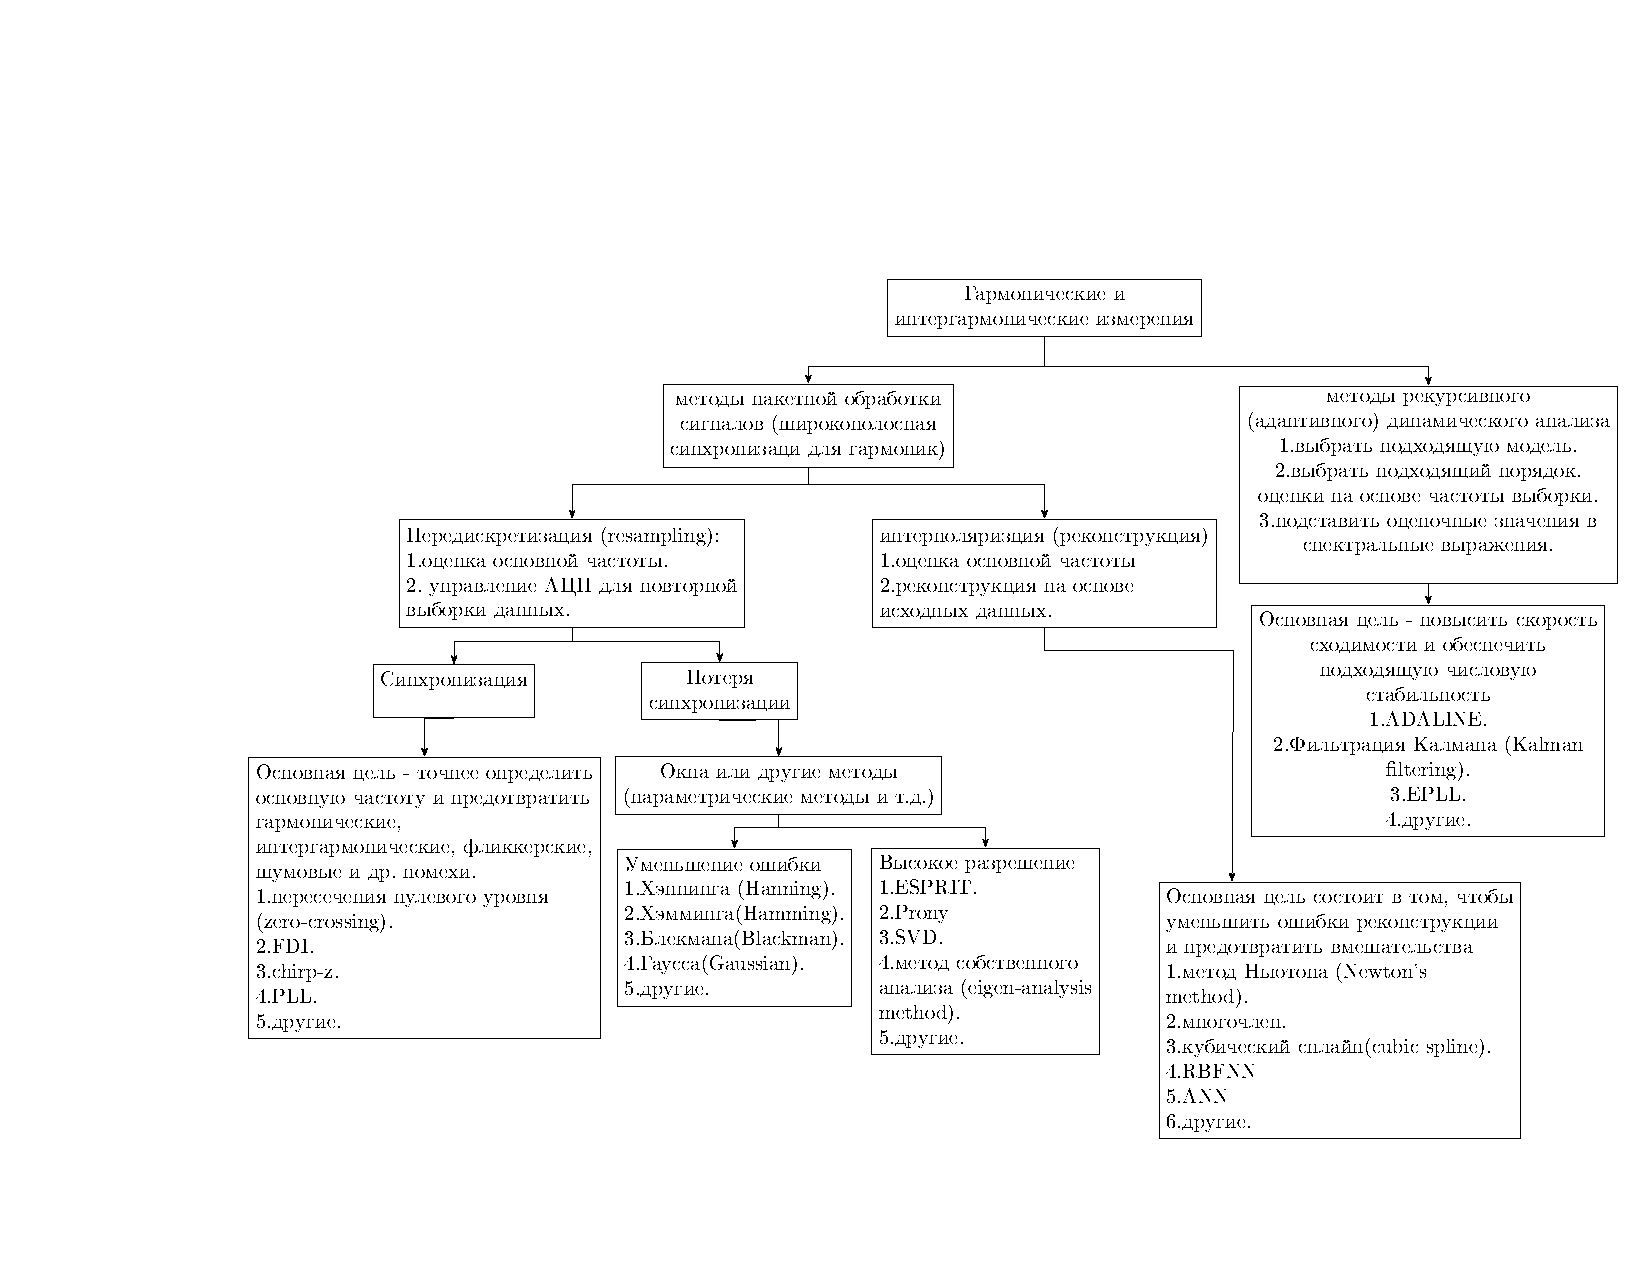
\includegraphics[scale=0.7]{picture15}
	}
	\caption{Упрощенная классификация обычно используемых методов гармонических и межгармонических оценок.}\label{fig:picture2}
\end{figure}



Сошлёмся на библиографию.
Одна ссылка: \cite[с.~54]{Sokolov}\cite[с.~36]{Gaidaenko}.
Две ссылки: \cite{Sokolov,Gaidaenko}.
Ссылка на собственные работы: \cite{vakbib1, confbib2}.
Много ссылок: %\cite[с.~54]{Lermontov,Management,Borozda} % такой «фокус»
%вызывает biblatex warning относительно опции sortcites, потому что неясно, к
%какому источнику относится уточнение о страницах, а bibtex об этой проблеме
%даже не предупреждает
\cite{Lermontov, Management, Borozda, Marketing, Constitution, FamilyCode,
Gost.7.0.53, Razumovski, Lagkueva, Pokrovski, Methodology, Nasirova, Berestova,
Kriger}%
\ifnumequal{\value{bibliosel}}{0}{% Примеры для bibtex8
    \cite{Sirotko, Lukina, Encyclopedia}%
}{% Примеры для biblatex через движок biber
    \cite{Sirotko2, Lukina2, Encyclopedia2}%
}%
.
И~ещё немного ссылок:~\cite{Article,Book,Booklet,Conference,Inbook,Incollection,Manual,Mastersthesis,
Misc,Phdthesis,Proceedings,Techreport,Unpublished}
% Следует обратить внимание, что пробел после запятой внутри \cite{}
% обрабатывается ожидаемо, а пробел перед запятой, может вызывать проблемы при
% обработке ссылок.
\cite{medvedev2006jelektronnye, CEAT:CEAT581, doi:10.1080/01932691.2010.513279,
Gosele1999161,Li2007StressAnalysis, Shoji199895, test:eisner-sample,
test:eisner-sample-shorted, AB_patent_Pomerantz_1968, iofis_patent1960}
\ifnumequal{\value{bibliosel}}{0}{% Примеры для bibtex8
}{% Примеры для biblatex через движок biber
    \cite{patent2h, patent3h, patent2}%
}%
.

\ifnumequal{\value{bibliosel}}{0}{% Примеры для bibtex8
Попытка реализовать несколько ссылок на конкретные страницы
для \texttt{bibtex} реализации библиографии:
[\citenum{Sokolov}, с.~54; \citenum{Gaidaenko}, с.~36].
}{% Примеры для biblatex через движок biber
Несколько источников (мультицитата):
% Тут специально написано по-разному тире, для демонстрации, что
% применение специальных тире в настоящий момент в biblatex приводит к непоказу
% "с.".
\cites[vii--x, 5, 7]{Sokolov}[v"--~x, 25, 526]{Gaidaenko}[vii--x, 5, 7]{Techreport},
работает только в \texttt{biblatex} реализации библиографии.
}%

Ссылки на собственные работы:~\cite{vakbib1, confbib1}

Сошлёмся на приложения: Приложение~\ref{app:A}, Приложение~\ref{app:B2}.

Сошлёмся на формулу: формула~\eqref{eq:equation1}.

Сошлёмся на изображение: рисунок~\ref{fig:knuth}.

Стандартной практикой является добавление к ссылкам префикса, характеризующего тип элемента.
Это не является строгим требованием, но~позволяет лучше ориентироваться в документах большого размера.
Например, для ссылок на рисунки используется префикс \textit{fig},
для ссылки на~таблицу "--- \textit{tab}.

В таблице~\ref{tab:tab_pref} приложения~\ref{app:B4} приведён список рекомендуемых
к использованию стандартных префиксов.

\section{Формулы}\label{sec:ch1/sec3}

Благодаря пакету \textit{icomma}, \LaTeX~одинаково хорошо воспринимает
в~качестве десятичного разделителя и запятую (\(3,1415\)), и точку (\(3.1415\)).

\subsection{Ненумерованные одиночные формулы}\label{subsec:ch1/sec3/sub1}

Вот так может выглядеть формула, которую необходимо вставить в~строку
по~тексту: \(x \approx \sin x\) при \(x \to 0\).

А вот так выглядит ненумерованная отдельностоящая формула c подстрочными
и надстрочными индексами:
\[
(x_1+x_2)^2 = x_1^2 + 2 x_1 x_2 + x_2^2
\]

Формула с неопределенным интегралом:
\[
\int f(\alpha+x)=\sum\beta
\]

При использовании дробей формулы могут получаться очень высокие:
\[
  \frac{1}{\sqrt{2}+
  \displaystyle\frac{1}{\sqrt{2}+
  \displaystyle\frac{1}{\sqrt{2}+\cdots}}}
\]

В формулах можно использовать греческие буквы:
%Все \original... команды заранее, ради этого примера, определены в Dissertation\userstyles.tex
\[
\alpha\beta\gamma\delta\originalepsilon\epsilon\zeta\eta\theta%
\vartheta\iota\kappa\varkappa\lambda\mu\nu\xi\pi\varpi\rho\varrho%
\sigma\varsigma\tau\upsilon\originalphi\phi\chi\psi\omega\Gamma\Delta%
\Theta\Lambda\Xi\Pi\Sigma\Upsilon\Phi\Psi\Omega
\]
\[%https://texfaq.org/FAQ-boldgreek
\boldsymbol{\alpha\beta\gamma\delta\originalepsilon\epsilon\zeta\eta%
\theta\vartheta\iota\kappa\varkappa\lambda\mu\nu\xi\pi\varpi\rho%
\varrho\sigma\varsigma\tau\upsilon\originalphi\phi\chi\psi\omega\Gamma%
\Delta\Theta\Lambda\Xi\Pi\Sigma\Upsilon\Phi\Psi\Omega}
\]

Для добавления формул можно использовать пары \verb+$+\dots\verb+$+ и \verb+$$+\dots\verb+$$+,
но~они считаются устаревшими.
Лучше использовать их функциональные аналоги \verb+\(+\dots\verb+\)+ и \verb+\[+\dots\verb+\]+.

\subsection{Ненумерованные многострочные формулы}\label{subsec:ch1/sec3/sub2}

Вот так можно написать две формулы, не нумеруя их, чтобы знаки <<равно>> были
строго друг под другом:
\begin{align}
  f_W & =  \min \left( 1, \max \left( 0, \frac{W_{soil} / W_{max}}{W_{crit}} \right)  \right), \nonumber \\
  f_T & =  \min \left( 1, \max \left( 0, \frac{T_s / T_{melt}}{T_{crit}} \right)  \right), \nonumber
\end{align}

Выровнять систему ещё и по переменной \( x \) можно, используя окружение
\verb|alignedat| из пакета \verb|amsmath|. Вот так:
\[
    |x| = \left\{
    \begin{alignedat}{2}
        &&x, \quad &\text{eсли } x\geqslant 0 \\
        &-&x, \quad & \text{eсли } x<0
    \end{alignedat}
    \right.
\]
Здесь первый амперсанд (в исходном \LaTeX\ описании формулы) означает
выравнивание по~левому краю, второй "--- по~\( x \), а~третий "--- по~слову
<<если>>. Команда \verb|\quad| делает большой горизонтальный пробел.



Ещё вариант:
\[
    |x|=
    \begin{cases}
    \phantom{-}x, \text{если } x \geqslant 0 \\
    -x, \text{если } x<0
    \end{cases}
\]

Кроме того, для  нумерованных формул \verb|alignedat| делает вертикальное
выравнивание номера формулы по центру формулы. Например, выравнивание
компонент вектора:
\begin{equation}
\label{eq:2p3}
\begin{alignedat}{2}
{\mathbf{N}}_{o1n}^{(j)} = \,{\sin} \phi\,n\!\left(n+1\right)
         {\sin}\theta\,
         \pi_n\!\left({\cos} \theta\right)
         \frac{
               z_n^{(j)}\!\left( \rho \right)
              }{\rho}\,
           &{\boldsymbol{\hat{\mathrm e}}}_{r}\,+   \\
+\,
{\sin} \phi\,
         \tau_n\!\left({\cos} \theta\right)
         \frac{
            \left[\rho z_n^{(j)}\!\left( \rho \right)\right]^{\prime}
              }{\rho}\,
            &{\boldsymbol{\hat{\mathrm e}}}_{\theta}\,+   \\
+\,
{\cos} \phi\,
         \pi_n\!\left({\cos} \theta\right)
         \frac{
            \left[\rho z_n^{(j)}\!\left( \rho \right)\right]^{\prime}
              }{\rho}\,
            &{\boldsymbol{\hat{\mathrm e}}}_{\phi}\:.
\end{alignedat}
\end{equation}

Ещё об отступах. Иногда для лучшей <<читаемости>> формул полезно
немного исправить стандартные интервалы \LaTeX\ с учётом логической
структуры самой формулы. Например в формуле~\ref{eq:2p3} добавлен
небольшой отступ \verb+\,+ между основными сомножителями, ниже
результат применения всех вариантов отступа:
\begin{align*}
\backslash! &\quad f(x) = x^2\! +3x\! +2 \\
  \mbox{по-умолчанию} &\quad f(x) = x^2+3x+2 \\
\backslash, &\quad f(x) = x^2\, +3x\, +2 \\
\backslash{:} &\quad f(x) = x^2\: +3x\: +2 \\
\backslash; &\quad f(x) = x^2\; +3x\; +2 \\
\backslash \mbox{space} &\quad f(x) = x^2\ +3x\ +2 \\
\backslash \mbox{quad} &\quad f(x) = x^2\quad +3x\quad +2 \\
\backslash \mbox{qquad} &\quad f(x) = x^2\qquad +3x\qquad +2
\end{align*}

Можно использовать разные математические алфавиты:
\begin{align}
\mathcal{ABCDEFGHIJKLMNOPQRSTUVWXYZ} \nonumber \\
\mathfrak{ABCDEFGHIJKLMNOPQRSTUVWXYZ} \nonumber \\
\mathbb{ABCDEFGHIJKLMNOPQRSTUVWXYZ} \nonumber
\end{align}

Посмотрим на систему уравнений на примере аттрактора Лоренца:

\[
\left\{
  \begin{array}{rl}
    \dot x = & \sigma (y-x) \\
    \dot y = & x (r - z) - y \\
    \dot z = & xy - bz
  \end{array}
\right.
\]

А для вёрстки матриц удобно использовать многоточия:
\[
\left(
  \begin{array}{ccc}
    a_{11} & \ldots & a_{1n} \\
    \vdots & \ddots & \vdots \\
    a_{n1} & \ldots & a_{nn} \\
  \end{array}
\right)
\]

\subsection{Нумерованные формулы}\label{subsec:ch1/sec3/sub3}

А вот так пишется нумерованная формула:
\begin{equation}
  \label{eq:equation1}
  e = \lim_{n \to \infty} \left( 1+\frac{1}{n} \right) ^n
\end{equation}

Нумерованных формул может быть несколько:
\begin{equation}
  \label{eq:equation2}
  \lim_{n \to \infty} \sum_{k=1}^n \frac{1}{k^2} = \frac{\pi^2}{6}
\end{equation}

Впоследствии на формулы~\eqref{eq:equation1} и~\eqref{eq:equation2} можно ссылаться.

Сделать так, чтобы номер формулы стоял напротив средней строки, можно,
используя окружение \verb|multlined| (пакет \verb|mathtools|) вместо
\verb|multline| внутри окружения \verb|equation|. Вот так:
\begin{equation} % \tag{S} % tag - вписывает свой текст
  \label{eq:equation3}
    \begin{multlined}
        1+ 2+3+4+5+6+7+\dots + \\
        + 50+51+52+53+54+55+56+57 + \dots + \\
        + 96+97+98+99+100=5050
    \end{multlined}
\end{equation}

Используя команду \verb|\labelcref| из пакета \verb|cleveref|, можно
красиво ссылаться сразу на несколько формул
(\labelcref{eq:equation1, eq:equation3, eq:equation2}), даже перепутав
порядок ссылок \verb|(\labelcref{eq:equation1, eq:equation3, eq:equation2})|.

Уравнения~(\labelcref{eq:subeq_1,eq:subeq_2}) демонстрируют возможности
окружения \verb|\subequations|.
\begin{subequations}
	\label{eq:subeq_1}
	\begin{gather}
		y = x^2 + 1 \label{eq:subeq_1-1} \\
		y = 2 x^2 - x + 1 \label{eq:subeq_1-2}
	\end{gather}
\end{subequations}
Ссылки на отдельные уравнения~(\labelcref{eq:subeq_1-1,eq:subeq_1-2,eq:subeq_2-1}).
\begin{subequations}
	\label{eq:subeq_2}
	\begin{align}
		y &= x^3 + x^2 + x + 1 \label{eq:subeq_2-1} \\
		y &= x^2
	\end{align}
\end{subequations}

\subsection{Форматирование чисел и размерностей величин}\label{sec:units}

Числа форматируются при помощи команды \verb|\num|:
\num{5,3};
\num{2,3e8};
\num{12345,67890};
\num{2,6 d4};
\num{1+-2i};
\num{.3e45};
\num[exponent-base=2]{5 e64};
\num[exponent-base=2,exponent-to-prefix]{5 e64};
\num{1.654 x 2.34 x 3.430}
\num{1 2 x 3 / 4}.
Для написания последовательности чисел можно использовать команды \verb|\numlist| и \verb|\numrange|:
\numlist{10;30;50;70}; \numrange{10}{30}.
Значения углов можно форматировать при помощи команды \verb|\ang|:
\ang{2.67};
\ang{30,3};
\ang{-1;;};
\ang{;-2;};
\ang{;;-3};
\ang{300;10;1}.

Обратите внимание, что ГОСТ запрещает использование знака <<->> для обозначения отрицательных чисел
за исключением формул, таблиц и рисунков.
Вместо него следует использовать слово <<минус>>.

Размерности можно записывать при помощи команд \verb|\si| и \verb|\SI|:
\si{\farad\squared\lumen\candela};
\si{\joule\per\mole\per\kelvin};
\si[per-mode = symbol-or-fraction]{\joule\per\mole\per\kelvin};
\si{\metre\per\second\squared};
\SI{1.2-3i e5}{\joule\per\mole\per\kelvin};
\SI{0.10(5)}{\neper};
\SIlist{1;2;3;4}{\tesla};
\SIrange{50}{100}{\volt}.
Список единиц измерений приведён в таблицах~(\labelcref{tab:unit:base,
tab:unit:derived,tab:unit:accepted,tab:unit:physical,tab:unit:other}).
Приставки единиц приведены в таблице~\ref{tab:unit:prefix}.

С дополнительными опциями форматирования можно ознакомиться в описании пакета \texttt{siunitx};
изменить или добавить единицы измерений можно в~файле \texttt{siunitx.cfg}.

\begin{table}
    \caption{Основные величины СИ.}\label{tab:unit:base}
    \centering
    \begin{tabular}{llc}
        \toprule
        Название  & Команда                & Символ         \\
        \midrule
        Ампер     & \verb|\ampere| & \si{\ampere}   \\
        Кандела   & \verb|\candela| & \si{\candela}  \\
        Кельвин   & \verb|\kelvin| & \si{\kelvin}   \\
        Килограмм & \verb|\kilogram| & \si{\kilogram} \\
        Метр      & \verb|\metre| & \si{\metre}    \\
        Моль      & \verb|\mole| & \si{\mole}     \\
        Секунда   & \verb|\second| & \si{\second}   \\
        \bottomrule
    \end{tabular}
\end{table}

\begin{table}
    \caption{Производные единицы СИ.}\label{tab:unit:derived}
    \small
    \centering
    \begin{tabular}{llc|llc}
        \toprule
        Название       & Команда                 & Символ              & Название & Команда & Символ \\
        \midrule
        Беккерель      & \verb|\becquerel|  & \si{\becquerel}     &
        Ньютон         & \verb|\newton|  & \si{\newton}                                      \\
        Градус Цельсия & \verb|\degreeCelsius| & \si{\degreeCelsius} &
        Ом             & \verb|\ohm| & \si{\ohm}                                         \\
        Кулон          & \verb|\coulomb| & \si{\coulomb}       &
        Паскаль        & \verb|\pascal| & \si{\pascal}                                      \\
        Фарад          & \verb|\farad| & \si{\farad}         &
        Радиан         & \verb|\radian| & \si{\radian}                                      \\
        Грей           & \verb|\gray| & \si{\gray}          &
        Сименс         & \verb|\siemens| & \si{\siemens}                                     \\
        Герц           & \verb|\hertz| & \si{\hertz}         &
        Зиверт         & \verb|\sievert| & \si{\sievert}                                     \\
        Генри          & \verb|\henry| & \si{\henry}         &
        Стерадиан      & \verb|\steradian| & \si{\steradian}                                   \\
        Джоуль         & \verb|\joule| & \si{\joule}         &
        Тесла          & \verb|\tesla| & \si{\tesla}                                       \\
        Катал          & \verb|\katal| & \si{\katal}         &
        Вольт          & \verb|\volt| & \si{\volt}                                        \\
        Люмен          & \verb|\lumen| & \si{\lumen}         &
        Ватт           & \verb|\watt| & \si{\watt}                                        \\
        Люкс           & \verb|\lux| & \si{\lux}           &
        Вебер          & \verb|\weber| & \si{\weber}                                       \\
        \bottomrule
    \end{tabular}
\end{table}

\begin{table}
    \caption{Внесистемные единицы.}\label{tab:unit:accepted}
    \centering
    \begin{tabular}{llc}
        \toprule
        Название        & Команда                 & Символ          \\
        \midrule
        День            & \verb|\day| & \si{\day}       \\
        Градус          & \verb|\degree| & \si{\degree}    \\
        Гектар          & \verb|\hectare| & \si{\hectare}   \\
        Час             & \verb|\hour| & \si{\hour}      \\
        Литр            & \verb|\litre| & \si{\litre}     \\
        Угловая минута  & \verb|\arcminute| & \si{\arcminute} \\
        Угловая секунда & \verb|\arcsecond| & \si{\arcsecond} \\ %
        Минута          & \verb|\minute| & \si{\minute}    \\
        Тонна           & \verb|\tonne| & \si{\tonne}     \\
        \bottomrule
    \end{tabular}
\end{table}

\begin{table}
    \caption{Внесистемные единицы, получаемые из эксперимента.}\label{tab:unit:physical}
    \centering
    \begin{tabular}{llc}
        \toprule
        Название                & Команда                 & Символ                 \\
        \midrule
        Астрономическая единица & \verb|\astronomicalunit| & \si{\astronomicalunit} \\
        Атомная единица массы   & \verb|\atomicmassunit| & \si{\atomicmassunit}   \\
        Боровский радиус        & \verb|\bohr| & \si{\bohr}             \\
        Скорость света          & \verb|\clight| & \si{\clight}           \\
        Дальтон                 & \verb|\dalton| & \si{\dalton}           \\
        Масса электрона         & \verb|\electronmass| & \si{\electronmass}     \\
        Электрон Вольт          & \verb|\electronvolt| & \si{\electronvolt}     \\
        Элементарный заряд      & \verb|\elementarycharge| & \si{\elementarycharge} \\
        Энергия Хартри          & \verb|\hartree| & \si{\hartree}          \\
        Постоянная Планка       & \verb|\planckbar| & \si{\planckbar}        \\
        \bottomrule
    \end{tabular}
\end{table}

\begin{table}
    \caption{Другие внесистемные единицы.}\label{tab:unit:other}
    \centering
    \begin{tabular}{llc}
        \toprule
        Название                  & Команда                 & Символ             \\
        \midrule
        Ангстрем                  & \verb|\angstrom| & \si{\angstrom}     \\
        Бар                       & \verb|\bar| & \si{\bar}          \\
        Барн                      & \verb|\barn| & \si{\barn}         \\
        Бел                       & \verb|\bel| & \si{\bel}          \\
        Децибел                   & \verb|\decibel| & \si{\decibel}      \\
        Узел                      & \verb|\knot| & \si{\knot}         \\
        Миллиметр ртутного столба & \verb|\mmHg| & \si{\mmHg}         \\
        Морская миля              & \verb|\nauticalmile| & \si{\nauticalmile} \\
        Непер                     & \verb|\neper| & \si{\neper}        \\
        \bottomrule
    \end{tabular}
\end{table}

\begin{table}
    \caption{Приставки СИ.}\label{tab:unit:prefix}
    \centering
    \small
    \begin{tabular}{llcc|llcc}
        \toprule
        Приставка & Команда                 & Символ      & Степень &
        Приставка & Команда                 & Символ      & Степень   \\
        \midrule
        Иокто     & \verb|\yocto| & \si{\yocto} & -24     &
        Дека      & \verb|\deca| & \si{\deca}  & 1         \\
        Зепто     & \verb|\zepto| & \si{\zepto} & -21     &
        Гекто     & \verb|\hecto| & \si{\hecto} & 2         \\
        Атто      & \verb|\atto| & \si{\atto}  & -18     &
        Кило      & \verb|\kilo| & \si{\kilo}  & 3         \\
        Фемто     & \verb|\femto| & \si{\femto} & -15     &
        Мега      & \verb|\mega| & \si{\mega}  & 6         \\
        Пико      & \verb|\pico| & \si{\pico}  & -12     &
        Гига      & \verb|\giga| & \si{\giga}  & 9         \\
        Нано      & \verb|\nano| & \si{\nano}  & -9      &
        Терра     & \verb|\tera| & \si{\tera}  & 12        \\
        Микро     & \verb|\micro| & \si{\micro} & -6      &
        Пета      & \verb|\peta| & \si{\peta}  & 15        \\
        Милли     & \verb|\milli| & \si{\milli} & -3      &
        Екса      & \verb|\exa| & \si{\exa}   & 18        \\
        Санти     & \verb|\centi| & \si{\centi} & -2      &
        Зетта     & \verb|\zetta| & \si{\zetta} & 21        \\
        Деци      & \verb|\deci| & \si{\deci}  & -1      &
        Иотта     & \verb|\yotta| & \si{\yotta} & 24        \\
        \bottomrule
    \end{tabular}
\end{table}
